%%
%% Dit is een subdocument van het projectplan.
%%
%%  hier worden tijden en eventueel personen toegekend aan activiteiten
%%


\subsection{Schedule}
 %% dit onderdeel moet vermoedelijk in het schedule plan
  

  \begin{figure}
  	\centering
  	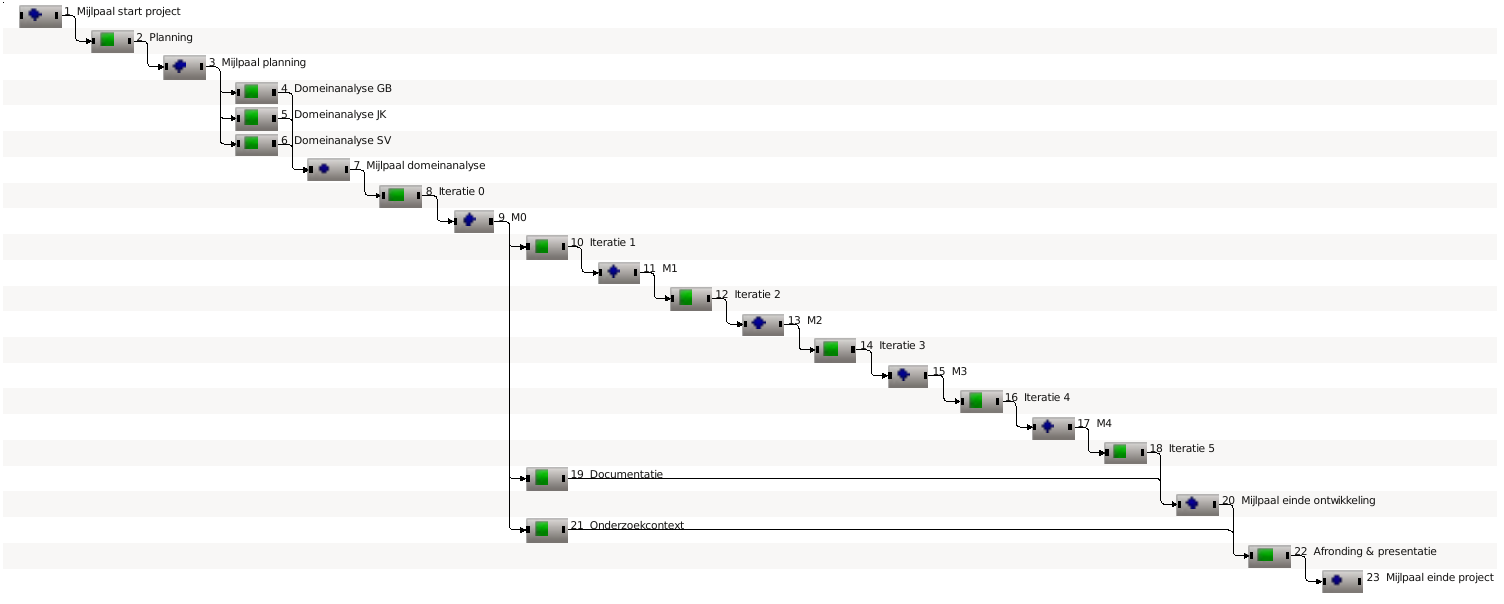
\includegraphics[width=0.8\textwidth,natwidth=1504,natheight=604]{Gantt.png}
  	\caption{\label{fig:Gantt Chart}Scheduling.}
  \end{figure}

\begin{tabular}{ll}\hline
{\bf Fase}    & {\bf weken}\\\hline
Planning             & 2,5 \\
\hline
Domeinanalyse        & 3 \\
Iteratie 0           & 3 \\
\hline
Iteratie 1           & 3 \\
Iteratie 2           & 3 \\
Iteratie 3           & 3 \\
Iteratie 4           & 3 \\
Iteratie 5           & 3 \\
\hline
Onderzoekcontext     &	2 \\
\hline
Afronding	     & 1.5 \\
\hline
Totaal               & 27 \\
\end{tabular}


\begin{itemize}
 \item 27 weken * 15 uur/week = 405 uur
 \item 8 maanden, ongeveer 32 weken beschikbaar, dus 5 weken marge
\end{itemize}



\begin{tabular}{lll}\hline
{\bf Week}    & {\bf Taak}  & {\bf Extra}\\\hline
38-41         & Planning    \\
42-45         & Domeinanalyse & 4 weken ingepland i.v.m. vakanties Stefan \& Jeroen \\
46-48         & Iteratie 0    \\
49-51         & Iteratie 1    \\
52-1          &               & geen iteratie i.v.m. vakantieperiode, mogelijk individueel (onderzoekcontext?) \\
2-4           & Iteratie 2    \\
5-7           & Iteratie 3    \\
8-10          & Iteratie 4    \\
11-13         & Iteratie 5    \\
14-16         &               \\
17-18         & Onderzoekcontext \\
19-20         & Afronding     \\
22            & Mijlpaal einde project

\end{tabular}




\paragraph{Capaciteitsplanning}

\begin{enumerate}
 \item vakanties?
 \item beschikbaarheid Freek en Bernard?
\end{enumerate}

\paragraph{Planning iteraties}
\begin{enumerate}
 \item 3 weken per interatie
 \item hoeveel tijd voor requirements?
 \item hoeveel tijd voor evaluatie?
\end{enumerate}